\documentclass[12pt]{article}
\usepackage[T1]{fontenc}
%\usepackage[latin9]{inputenc}
\usepackage[utf8]{inputenc}
\usepackage[english]{babel}
\usepackage{amsmath}
\usepackage{amsfonts}
\usepackage{amssymb}
\usepackage{setspace}
\usepackage{rotating}
\usepackage{graphics}
\usepackage[round]{natbib}
%\usepackage{graphicx}
%\usepackage{float} 				%allows you to float images
\usepackage{latexsym}
\usepackage{bbding}
%\usepackage {moresize}
\usepackage{listings}
\usepackage{bbding}
\usepackage{blindtext}
\usepackage{hhline}
%\usepackage{tikz}
%\usetikzlibrary{shapes,backgrounds}
%\usepackage{pgfplots}
%\usetikzlibrary{arrows}
\usepackage{enumitem}
\doublespacing
%\usepackage{geometry}
\usepackage{amsthm}
\usepackage{color}
%\usepackage{array,multirow}
%\usepackage{subcaption}
%\usepackage{pst-plot}
%	\psset{xunit=15mm}
%\geometry{verbose,tmargin=1in,bmargin=1in,lmargin=1in,rmargin=1in}
\setlength{\parskip}{\bigskipamount}
\setlength{\parindent}{0pt}

\newenvironment{problem}[2][Problem]{\begin{trivlist}
\item[\hskip \labelsep {\bfseries #1}\hskip \labelsep {\bfseries #2.}]}{\end{trivlist}}

\title{Problem Set 6 \thanks{Problem list 4.2.12, 4.2.28, 4.3.14, 4.4.6, 4.6.6}}
\author{Ian McGroarty \\
	Course Number: 625.603}
\date{March 14, 2019}

\begin{document}

\maketitle
\newpage
\begin{problem}{4.2.12} 
By Theorem 4.2.2 (pg 224) the random variable X is said to have a Poisson distribution if
$$ 
p_X(k) = P(X=k)=\frac{e^{-\hat{k}} \hat{k}^k}{k!}
$$
Let X denote the number of bags lost. The first two columns of Table 1 show the distribution of X for the 40 week period in question. Here the average number of bags lost, $\hat{k} = 1.525$. The last two columns of Table 1 compare the observed prooportions of bags lost for which X=k with the prosed Poisson model
$$ p_X(k) = e^{-1.525}\frac{(1.525)^k}{k!}, \ k=0,1,2,3,4,5 $$
There is a fairly close agreement between the two columns. Thus, the number of bags lost in a given week can be considered a Poisson random variable. 
\begin{table}[h!]
	\begin{center}
	\caption{Table 1}
	\begin{tabular}{l|ccc}
Bags Lost, $k$	& Frequency	& Porportion	& $p_X(k)$ \\
\hline
0 &	9	& 0.225		& 0.218 \\
1&	13	&0.325		&0.332 \\
2&	10	&0.25		&0.253 \\
3&	5	&0.125		&0.128 \\
4&	2	&0.05		&0.049 \\
5&	1	&0.025		&0.015 \\
\hline
  &	40	&1 			&1 \\
	\end{tabular}
	\end{center}
\end{table}
\end{problem} 

\newpage

\begin{problem}{4.2.28}
Since lightbulbs go out independently of one another, and occur at a constant rate $\lambda $ we can say that the occurance of light bulbs going out are Poisson events. By Theorem 4.2.3 (pg 233), we can say that the pdf describig the distribution of intervals between events should have the exponential form: $f_Y(y) = \lambda e^{-\lambda y}$. At a burn out rate of 1.1 bulbs per one hundred hours, $\lambda = \frac{1.1 \ bulbs}{100 \ hours}= 0.011$ Thus, $f_Y(y) = 0.011 e^{-0.011 y}$ We want to find $P(y < 75)$.\footnote{I need to be honest here. For this integration, I followed example 4.2.5. I do not fully understand how we can make a u substitution and have that never come back into play. Or how we move the 0.011 * 75 the the bottom of the integral. I assume the two operations are related but I do not see how this is okay.} 
\begin{align*}
P(y<75) &= 1- P(y>75) && \text{Theorem 2.3.1 (pg 27)} \\
&= 1 - \int_{75}^{\infty}( 0.011 e^{-0.011 y}dy) && \text{Theorem 4.2.3 (pg 233)} \\
&= 1 - \int_{0.825}^{\infty}e^{-u}du && \text{let $u = 0.011y$} \\
&=1 -e^{-u}\Big|_{0.825}^{\infty} = 1 - e^{-0.825} \\
P(y<75) &= 0.562 \\
E(Y) &= np && \text{Theorem 3.5.1 (pg 139)\footnotemark} \\
&=50 \ bulbs \cdot 0.562 = 28.1 \ bulbs
\end{align*}
\footnotetext{I couldn't find anything to generalize this from the discrete case but I know that it works}
\end{problem}
 \newpage

\begin{problem}{4.3.14}
\begin{figure}
  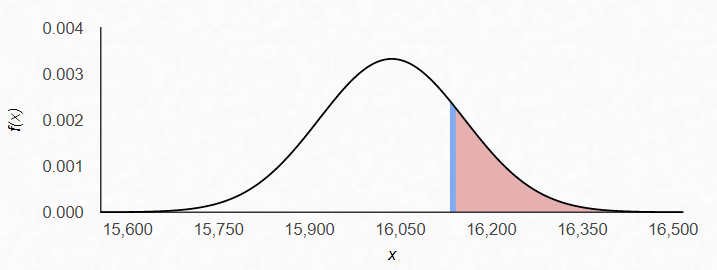
\includegraphics[width=\linewidth]{4-3-14.png}
  \caption{Figure 1}
  \label{fig:boat1}
\end{figure}
Let X denote the number of hot dogs sold at the game.  While in practice people buy hot dogs in groups, we can approximate by assuming that X is binomial with n=42,200 and p = 0.38.  Let $\hat{x}$ be the expected number of hot dogs that will be sold at next Tuesday's game (number of hot dogs to buy) such that $P(X>\hat{x}) \leq 0.2$ Equivalently (by completeness),   $P(X<\hat{x}) < 0.8$. Figure 1 shows the probability distribution of X, where the shaded region represents the area of p=0.2 where demand exceeds supply, and the blue line is $\hat{x}$. Using table 4.2.1 (pg 238) we see that a probability of 0.8 is associated with a Z statistic of 0.84 (probability 0.7995 is closest to 0.8 with price is right rules). By Theorem 4.3.1 (pg 237) and the continuity correction (pg 240), 
\begin{align*}
P(X<\hat{x}) &= P[\frac{X-np}{\sqrt{np(1-p)}} < \frac{\hat{x}+0.5 -np}{\sqrt{np(1-p)}}]
&= P[Z < \frac{\hat{x}+0.5 -(42200)(0.38)}{\sqrt{(42200)(0.38)(1-0.38)}}] \\
&=  \frac{\hat{x}+0.5 -(42200)(0.38)}{\sqrt{(42200)(0.38)(1-0.38)}} = 0.84 \\
\hat{x} &= 16120.26
\end{align*}
\end{problem}

\begin{problem}{4.4.6} 
3 dice may sum to 4 if there is some combination of (1,1,2). This gives 3 potential successes of $6^3 = 216$ possibly outcomes. Let the random variable X be the trial at which the first success occurs with $p = \frac{3}{216}={1}{72}$. Each dice roll is an independent trial, with either a possibility of either success or failure, thus X is a geometric random variable. Using the result of Question 4.4.5, we can say that the cdf of X is given by $F_X(t) = P(X \leq t) = 1 - (1-p)^t$. 
\begin{align*} 
P(65\leq X \leq 75) &= F_X(75)-F_X(65) && \text{Theorem 3.4.2 (pg 135)\footnotemark} \\
&= [1-(1-\frac{1}{72})^{75}] - [1-(1-\frac{1}{72})^{65}] \\
P(65\leq X \leq 75) &=0.052
\end{align*}
\footnotetext{Generalized in the discrete case on page 125}
\end{problem}

\newpage
\begin{problem}{4.6.6}Show that $\Gamma (1/2) = \sqrt{\pi }$
\begin{align*}
\Gamma(r) &= \int_0^{\infty} y^{r-1}e^{-y}dx  && \text{Definition 4.6.1 (pg 268)} \\
\Gamma(r) &= 2\int_0^{\infty} x^{2r-1}e^{-x^2}dx  && \text{Let y =$x^2$} \\
\Gamma(1/2) &=2 \int_0^{\infty} e^{-x^2}dx  &&\text{Gaussian integral\footnotemark} \\
\Gamma(1/2) &= \sqrt{\pi }
\end{align*}
\footnotetext{$https://en.wikipedia.org/wiki/Gaussian_integral$}
\end{problem}
\end{document}

http://jekyll.math.byuh.edu/courses/m321/handouts/gammahalf.pdf
https://studylib.net/doc/18411298/proof-of-gamma-1-2-